\documentclass[./../../paper.tex]{subfiles}
\graphicspath{{\subfix{./../../figures/}}}

\begin{document}

\section{Determine the Evolutionary Algorithm Hyperparameter settings}

\subsection{Experimental Setup}
\label{sec:exp2}
Given the combinatory set of configurations chosen in \autoref{sec:exp1}, we will explore optimal parameter setting. Therefore, we run each configuration with a multitude of different hyperparameter settings.

For each configuration we vary the mutation rates and edit rates. The mutation rates for every edit-type are each between 0 and 1 and sum to 1. For the edit rate we explore values between 0.1 and 0.9. We do not, explore the extremes for the edit-rate as this would amount to either never changing the sequence or completely changing the sequence. An edit-rate of 0 would translate to never changing the sequence. This conflicts with the very core of generating counterfactuals. An edit-rate of 1 amounts to changing the complete sequence, which makes the convergence to an optimum impossible.

We use the resulting viability and feasibility as dependent variables and each hyperparameter edit-type in interaction with edit-rate as independent variable.

Furthermore, it confilicts with the Sparcity and Similarity criterions. The remaining procedure follows the process described in \autoref{sec:exp1}.


\subsection{Results}
\attention{Correlation matrix makes no sense. It should be only a bar plot with feasibility and viability with all the hyperparams.}

\begin{figure}
    \centering
    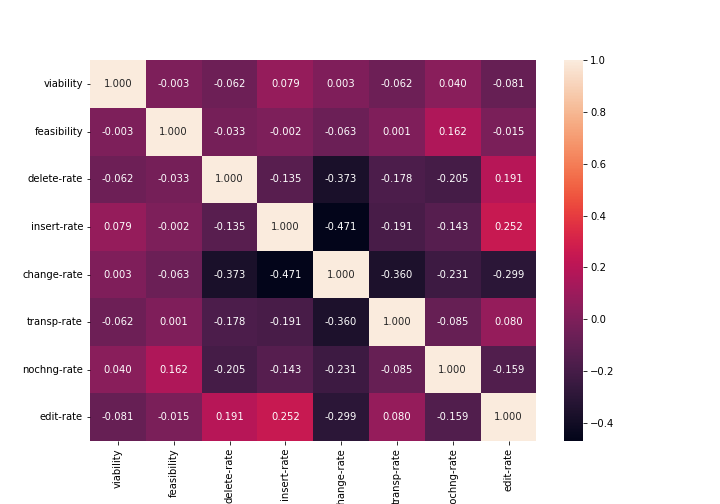
\includegraphics[width=\textwidth]{figures/results/params_heatmap.png}
    \caption{Shows a correlation matrix of each hyperparameter, the feasibility measure and the viability measure.}
    \label{fig:param_results_1}
\end{figure}

\autoref{fig:param_results_1} suggests that all hyperparamers have a negative correlation with feasibility and viability. Even, if we consider the interaction with edit-rate. The edit-rate itself appears to be beneficial. 


\begin{table}
    \caption{Table shows the result of the linear mixed model. It uses viability as dependent variable and the hyperparameters as independent numerical variables. The model is adjusted for general differences in indivdual hyperparameter settings.}
    \label{tbl:params_viability}
    \begin{tabular}{llll}
                               & Coef.  & Std.Err. & p-value \\
        Intercept              & 2.523  & 0.069    & 0.000   \\
        erate                  & 0.009  & 0.011    & 0.443   \\
        erate:dmrate           & -0.158 & 0.012    & 0.000   \\
        erate:imrate           & -0.009 & 0.012    & 0.463   \\
        erate:cmrate           & -0.072 & 0.011    & 0.000   \\
        erate:tmrate           & -0.196 & 0.011    & 0.000   \\
        Hyperparameter Set Var & 0.029  & 0.114    &         \\
    \end{tabular}
\end{table}

If we inspect the model results in terms of viability \autoref{tbl:params_viability}, we see a similar trend. Furthermore, it appears, that the specific hyperparameter set affects the results positively. This suggests, that the edit-rate might be the most important hyperparameter. Secondly, we can assume that a carefully chosen balance in hyperparameters to achieve an increase in viability.   

\begin{table}
    \caption{Table shows the result of the linear mixed model. It uses feasibility as dependent variable and the hyperparameters as independent numerical variables. The model is adjusted for general differences in indivdual hyperparameter settings.}
    \label{tbl:params_feasibility}
    \begin{tabular}{llll}
     & Coef. & Std.Err. & p-value \\
    Intercept & 0.022 & 0.011 & 0.041 \\
    erate & 0.099 & 0.004 & 0.000 \\
    erate:dmrate & -0.105 & 0.004 & 0.000 \\
    erate:imrate & -0.105 & 0.004 & 0.000 \\
    erate:cmrate & -0.107 & 0.004 & 0.000 \\
    erate:tmrate & -0.102 & 0.004 & 0.000 \\
    Hyperparameter Set Var & 0.001 & 0.009 &  \\
    \end{tabular}
\end{table}

% \needstbl{tbl:feasibility_params}{This table shows the results of the mixed linear model using feasibility as dependent variable.}

Looking at feasibility in \autoref{tbl:params_feasibility}, we see the same behavior. However, the models defined in this section only explain linear behaviours. Hence, \autoref{fig:parameter_effects}, show each individual effect in relation to viability.

\begin{figure}
    \centering
    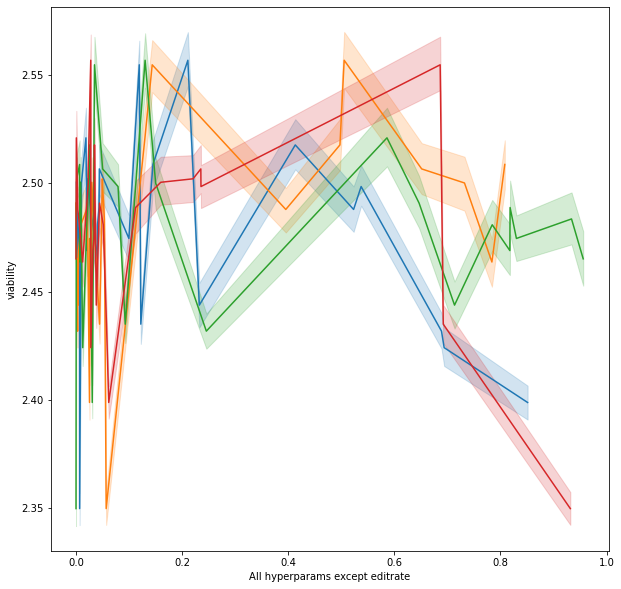
\includegraphics[width=\textwidth]{figures/results/result_params.png}
    \caption{Shows all 4 edit-types and their effect on viability.}
    \label{fig:parameter_effects}
\end{figure}

\autoref{fig:parameter_effects} indeed shows that the edit-types highly fluctuate in their effect on viability. These results suggest that the linear models do not accurately reflect the effect of each of the edit-types. \xixi{I know this plot looks horrible. I am sorry, I could't polish it on time.}

\subsection{Discussion}
\xixi{This section may not be correct anymore as I couldn't manage to rerun the experiment on time. These remarks are based on older results.}
The result is reasonable, as most counterfactuals that differ from the initial factual have never been seen in the dataset. Therefore, they are deemed impossible by the feasibility measure. With this in mind, we opt to choose the set of hyperparameters that increase the chance of finding feasible counterfactuals by averaging the hyperparamers of the non-zero feasibility subset. This selection most likely deacreases viability, but this is prefered over impossible counterfactuals.

Therefore, we choose \attention{a set of specific hyperparameter values} for any subsequent experiment.

\end{document}